\chapter{Propagazione di un Segnale a Banda Stretta}
Analizziamo la \textbf{propagazione} di un segnale a \textbf{banda} \textbf{stretta}.\\ \\
Facciamo prima alcune considerazioni sulla \textbf{Trasformata di Fourier}:
\begin{squared}[violet]
\tag{Trasformata}
    S (\w) = \int_{- \infty}^{\infty} s (t) e^{-j\w t} dt
\end{squared}
\begin{squared}
\tag{Antitrasformata}
    s (t) = \frac{1}{2\pi} \int_{- \infty}^{\infty} S (\w) e^{j\w t} d\w = \int_{- \infty}^{\infty} S (2\pi f) e^{j2\pi f t}
\end{squared}
E considerando un segnale $s(t)$ \textbf{reale}, possiamo dire che:
\begin{equation*}
    s(t) = s^*(t) \leftrightarrow S^*(\w) = \int_{- \infty}^{\infty} s(t) e^{j\w t} dt = S(-\w)
\end{equation*}
Questo ci fa capire che per rappresentare un segnale ci basta considerare le \textbf{sole pulsazioni positive}, infatti:
\begin{equation*}
\begin{aligned}
    s(t) &= \frac{1}{2\pi} \int_{- \infty}^{\infty} S(\w) e^{j\w t} d\w = \\
    &= \frac{1}{2\pi} \int_{0}^{\infty}S(\w) e^{j\w t} d\w +\frac{1}{2\pi} \int_{- \infty}^{0}S(\w)e^{j\w t} d\w  = \\
    &\boxed{\w'= -\w \quad d\w' = -d\w}\\
    &= \frac{1}{2\pi} \int_{0}^{\infty} S(\w) e^{j\w t} d\w  + \color{blue}{\frac{1}{2\pi} \int_{0}^{\infty} S(-\w') e^{-j\w' t} d\w'}
\end{aligned}
\end{equation*}
Quindi sfruttando quanto detto:
\begin{equation*}
     \color{blue}{\int_{0}^{\infty} S(-\w') e^{-j\w' t} d\w'} \color{black}{ =  \int_{0}^{\infty} S{(\w')}^* e^{-j\w' t} d\w' = {\left[\int_{0}^{\infty} S(\w') e^{j\w' t} d\w'\right]}^*}
\end{equation*}
Che possiamo sostituire sopra, ottenendo:
\begin{equation*}
    \begin{aligned}
    s(t) &= \frac{1}{2\pi} \int_{- \infty}^{\infty} S(\w) e^{j\w t} d\w = \\
    &= \frac{1}{2\pi} \int_{0}^{\infty}S(\w) e^{j\w t} d\w +\frac{1}{2\pi} \int_{0}^{\infty}S(-\w')e^{j\w' t} d\w' =\\
    &= \frac{1}{2\pi} \int_{0}^{\infty}S(\w) e^{j\w t} d\w + \frac{1}{2\pi} {\left[\int_{0}^{\infty} S(\w') e^{j\w' t} d\w'\right]}^* =\\
    &= 2Re\left\{\frac{1}{2\pi} \int_{0}^{\infty}S(\w) e^{j\w t} d\w  \right\} = Re\left\{\frac{1}{2\pi} \int_{0}^{\infty} 2 S(\w) e^{j\w t} d\w  \right\}
    \end{aligned}
\end{equation*}
\textbf{Definisco ora:}
\begin{equation*}
    \begin{dcases}
    \hat{S}(\w) = 2 S(\w) \quad per \quad \w > 0 \\
    \hat{S}(\w) = 0 \quad per \quad \w < 0 \\
    \end{dcases}
    \leftrightarrow \hat{s}(t) = \frac{1}{2\pi}\int_{- \infty}^{\infty}  \hat{S}(\w) e^{j\w t} d\w  
\end{equation*}
In particolare:
\begin{equation*}
    s(t) = Re\{\hat{s}(t)\} \quad \textbf{\LARGE $\hat{s} (t)$ è detto segnale analitico}
\end{equation*}
Analizziamo ora la \textbf{propagazione} di un segnale a \textbf{banda} \textbf{stretta} lungo la seguente linea:
\begin{center}
    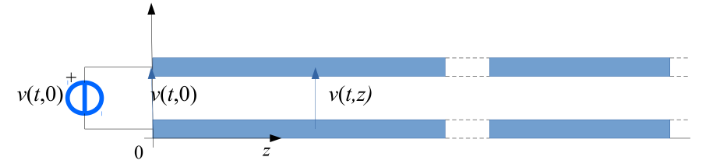
\includegraphics[width=.8\textwidth]{Images/figure27.png}
\end{center}
Scriviamo $v(t,0)$ così:
\begin{equation*}
    v(t,0) = s(t) \cos(\w_0 t)
\end{equation*}
In particolare:
\begin{itemize}
    \item $s(t) = s_0$ per $|t| < \frac{\tau}{2}$
     \item $s(t) = 0$ per $|t| > \frac{\tau}{2}$
     \item $\w_0 >> \frac{2\pi}{\tau}$
\end{itemize}
Il segnale $v(t, 0)$ è \textbf{reale} e a \textbf{banda} \textbf{stretta}, quindi procediamo associandogli il suo \textbf{analogo nella frequenza} e il suo \textbf{segale analitico}:
\begin{equation*}
    \tag{Analogo in Frequenza}
\begin{aligned}
    V(\w, 0) &= \int_{- \infty}^{\infty} v(t, 0)e^{-j\w t} dt = \\
    &= \int_{- \infty}^{\infty}s(t) \cos(\w_0 t)e^{-j\w t} dt = \\
    &=\frac{1}{2}\int_{- \infty}^{\infty} s(t) \left(e^{j\w_0 t} + e^{-j\w_0 t}\right)e^{-j\w t} dt
\end{aligned}
\end{equation*}

\begin{equation*}
    \tag{Segnale Analitico}
    \hat{V}(\w, 0) = \int_{- \infty}^{\infty} s(t) e^{j\w_0 t} e^{-j\w t} dt = \int_{- \infty}^{\infty} s(t) e^{-j(\w -\w_0)t}dt = S(\w - \w_0)
\end{equation*}

Quindi ora possiamo analizzare il problema nel dominio della frequenza:\\ \\
Fissato $\w$:
\begin{equation*}
    \hat{V}(\w, z) = \hat{V} (\w, 0) e^{-j \beta z}
\end{equation*}
Passiamo nel \textbf{dominio del tempo}:
\begin{equation*}
    \hat{v}(t, z) = \frac{1}{2\pi} \int_{- \infty}^{\infty}\hat{V}(\w, 0) e^{j \w t} e^{-j\beta z} d\w
 \end{equation*}

Distinguiamo ora i casi di \textbf{linea non dispersiva} e \textbf{linea dispersiva}.\\ \\
\section{Linea Non Dispersiva}
\begin{equation*}
    \beta(\w) = \w \sqrt{LC} = \w \sqrt{\epsilon \mu} = \frac{\w}{c}
\end{equation*}
dove $c = {\left(\frac{d\beta}{d\w}\right)}^{-1} = \frac{\w}{\beta}$.\\ \\
Facciamo la \textbf{sostituzione} in $\hat{v}(t,z)$:
\begin{equation*}
    \begin{aligned}
    \hat{v}(t,z) &= \frac{1}{2\pi} \int_{- \infty}^{\infty}\hat{V}(\w, 0) e^{j\w t} e^{-j \frac{\w}{c}z} d\w = \\
    &= \frac{1}{2\pi} \int_{- \infty}^{\infty}\hat{V}(\w, 0) e^{j\w \left( t - \frac{z}{c}\right)} d\w \\
    & t_R = t - \frac{z}{c} \\
    &\implies = \frac{1}{2\pi} \int_{- \infty}^{\infty}\hat{V}(\w, 0)e^{j\w t_R}  d\w = \\
    &= \hat{v}(t_R, 0) = \hat{v}\left(t - \frac{z}{c}, 0\right) = s\left(t - \frac{z}{c}\right) e^{j \w_0 \left(t - \frac{z}{c}\right)}
    \end{aligned}
\end{equation*}
Mentre $v(t,z)$ sarà:
\begin{equation*}
    v(t,z) = Re\{\hat{v}(t,z)\} = s\left(t - \frac{z}{c}\right) \cos\left(\w_0 \left(t - \frac{z}{c}\right)\right)
\end{equation*}
Quindi se la linea non è dispersiva,\textbf{ il segnale si propaga senza dispersione}.

\section{Linea Dispersiva}
In questo caso $\epsilon$ e $\mu$ sono \textbf{funzioni} di $\w$, o siamo in una situazione \textbf{NON TEM} ($\beta$ non è una funzione lineare di $\w$).\\ \\

Detta $\Delta \w$ la \textbf{banda del segnale} centrato in $\w_0$:
\begin{equation*}
    \begin{aligned}
    \hat{v}(t,z) &= \frac{1}{2\pi} \int_{- \infty}^{\infty}\hat{V}(\w, 0)e^{j\w t}e^{-j\beta z} d\w = \\
    &= \frac{1}{2\pi} \int_{\w_0 - \Delta \w}^{\w_0 + \Delta \w}\hat{V}(\w, 0)e^{j\w t}e^{-j\beta z} d\w 
    \end{aligned}
\end{equation*}
Questo ci fa capire che per calcolare $\hat{v}(t,z)$ ci servono i valori di $\beta$ solo \textbf{intorno} a $\w_0$.\\ \\
Quindi svilupperemo $\beta$ in \textbf{serie di Taylor} centrato in $\w_0$:
\begin{equation*}
    \beta(\w) = \beta_0 + \beta'_0(\w -\w_0) + \frac{1}{2} \beta''_0 (\w - \w_0)^2 + ...
\end{equation*}
Quindi:
\begin{equation*}
    \begin{aligned}
    \hat{v}(t,z) &=  \frac{1}{2\pi} \int_{- \infty}^{\infty}\hat{V}(\w, 0)e^{j\w t}e^{-j\beta z} d\w = \\
    &= \frac{1}{2\pi} \int_{- \infty}^{\infty}\hat{V}(\w, 0)e^{j\w t}e^{-j(\beta_0 + \beta'_0(\w -\w_0)) z} d\w = \\
    &= \frac{1}{2\pi} \int_{- \infty}^{\infty}\hat{V}(\w, 0)e^{j(\w t - \beta_0 z - \beta'_0(\w -\w_0)z )} d\w\\
    &\Omega = \w - \w_0\\
    &= \frac{1}{2\pi} \int_{- \infty}^{\infty}\hat{V}(\Omega + \w_0 , 0) e^{j(\Omega t + \w_0 t - \beta_0 z - \beta'_0\Omega z )} d\w = \\
    &= e^{(j(\w_0 t - \beta_0 z))} \frac{1}{2\pi} \int_{- \infty}^{\infty}\hat{V}(\Omega + \w_0 , 0) e^{j(\Omega t - \beta'_0 \Omega z)} d\w
    \end{aligned}
\end{equation*}
Dove:
\begin{equation*}
    \hat{V}(\Omega + \w_0, 0) = S(\Omega)
\end{equation*}
Dato che:
\begin{equation*}
    \hat{V}(\w, 0) = S(\w - \w_0)
\end{equation*}
Poniamo:
\begin{equation*}
    t_R = t - \beta'_0 z
\end{equation*}
Quindi:
\begin{equation*}
\begin{aligned}
    \hat{v}(t,z) &= e^{j( \w_0 t - \beta_0 z)} \frac{1}{2\pi} \int_{- \infty}^{\infty} S(\Omega, 0) e^{j \Omega t_R} d\Omega = \\
    &= e^{j(\w_0 t - \beta_0 z)} s(t_R) = e^{j(\w_0 t - \beta_0 z)} s(t - \beta'_0 z)
\end{aligned}
\end{equation*}
Definiamo:
\begin{itemize}
    \item \textbf{Velocità di Fase}: $\nu_F = \frac{\w_0}{\beta_0}$ alla pulsazione $\w_0$
    \item \textbf{Velocità di Gruppo}: $\nu_G = \frac{1}{\beta'_0}$ alla pulsazione $\w_0$
\end{itemize}
Sostituiamo:
\begin{squared}[green]
    \hat{v}(t,z) = \underbrace{e^{j\w_0 \left(t - \frac{z}{\nu_F}\right)}}_{Portante} \underbrace{s\left(t - \frac{z}{\nu_G}\right)}_{Inviluppo}
\end{squared}
Dove l'\textbf{Inviluppo} è l'\textbf{energia del segnale che si propaga lungo la linea a velocità} $\nu_G$.\\ \\
Quindi è identico al caso non dispersivo, tuttavia solo per brevi distanze, dato che per distanze più lunghe bisogna considerare ordini superiori dello sviluppo di Taylor di $\beta(\w)$.\\ \\
\subsection{Grado di Correttezza}
Per \textbf{quantificare il grado di correttezza dell'approssimazione} dobbiamo controllare se:
\begin{equation*}
    \frac{e^{-j\beta z}}{e^{-j(\beta_0 + \beta'_0 (\w - \w_0))z}} = e^{-j (\beta - \beta_0 - \beta'_0 (\w - \w_0))} \approx 1
\end{equation*}
Quindi possiamo procedere sviluppando $\beta$:
\begin{equation*}
\begin{aligned}
        (\beta_0 + \beta'_0 (\w - \w_0) &+ \frac{1}{2}\beta''_0 (\w - \w_0)^2 + ... - \beta_0 - \beta'_0 (\w - \w_0) )z = \\
        &=(\frac{1}{2} \beta''_0 (\w - \w_0)^2 + ...)z
\end{aligned}
\end{equation*}
Ora sostituendo:
\begin{equation*}
    e^{-j(\beta - \beta_0 - \beta'_0 (\w - \w_0))z} = e^{-j(\frac{1}{2} \beta''_0(\w - \w_0)^2 + ...)z} \approx 1
\end{equation*}
Che è verificata se e solo se:
\begin{equation*}
    \left|\left(\frac{1}{2} \beta''_0(\w - \w_0)^2 + ...\right)z\right| <<1
\end{equation*}
Quindi è evidente che \textbf{al crescere della distanza} (z) \textbf{questa disuguaglianza non sarà più verificata}.\\ \\

Possiamo avere una \textbf{stima della distanza} prima della quale è verificata se vale:
\begin{equation*}
    \left|\frac{1}{2} \beta''_0(\w - \w_0)^2 z \right| << 1
\end{equation*}
Ovvero: 
\begin{equation*}
    |z| << \frac{1}{ \left|\frac{1}{2} \beta''_0(\Delta \w)^2 \right|} = L_0
\end{equation*}















































%\chapter{Risonanze}
%\section{Circuito Risonante Serie}
%\section{Circuito Risonante Parallelo}
%\section{Circuito Risonante con Perdite}
%\section{Capacità Filtranti di un Risuonatore}
%\section{Risuonatori a Parametri Distribuiti}
%\subsection{Calcolo di Q}
%
%\chapter{Parametri dei Cavi Coassiali}
%\section{Calcolo del Campo Elettrico}
%\section{Calcolo di C}
%\section{Calcolo di L}
%\section{Calcolo di H}
%\section{Adattamento con Inverter}